In this chapter, we will explain the fundamentals and technologies that have been used for the experimentation. We will focus on three main aspects:
\begin{enumerate}
\item The used dataset.
\item The used libraries for the development of the code.
\item Analysis of the code itself.
\item The used metrics to evaluate the obtained results.
\end{enumerate}

The idea of the experimentation part is to test and compare the frameworks that we have presented in Chapters \ref{Chapter:SimCLR} and \ref{Chapter:BYOL}. Their architectures have already been explained, and the original code for both backbones has not been done by me. 

This work will focus on testing how changing the training hyperparameters of the model affects the final results, since the original papers \cite{chen_simple_2020,grill2020bootstrap} already mention that using their structure, the results are affected by those hyperparameters, such as batch size, network depth or network width.

The implementations that have been used can be found in:
\begin{itemize}
\item SimCLR implementation: Official implementation from Google in \url{https://github.com/google-research/simclr/tree/master/tf2}

\item BYOL implementation: not official, found in \url{https://github.com/garder14/byol-tensorflow2}. 
\end{itemize}

Although there exists an official implementation of BYOL, non-official one has been chosen because it uses \emph{Tensorflow}, which makes the implementations easier to understand and modify, which we needed to do. Also, the idea is to make use of \emph{Tensorboard}, a Tensorflow utility that helps with visualization and graph generation of the training and final results.


\section{Hardware and basic libraries}

When running training experiments in DL, the used hardware is one of the most determining factors for the results obtained by the models. There are many reasons for this, such as the time spent on the training a model or the amount of  data that we can fit in the GPUs (which will be our case) or TPUs.

For the experiments of this project, the DECSAI\footnotemark department of the University of Granada generously provided us access to a server that has a few NVIDIA GeForce RTX 3090. This model of GPU is one of the best in the market, having a \emph{compute capability} of $8.6/10$, rated by the NVIDIA company. IT also has a memory of $24GB$, which allows us to experiment with relatively large batch sizes using a single GPU and not having to parallelize the experiment.

%------------- Footnotemark
\footnotetext{The DECSAI's website is \url{https://decsai.ugr.es/}.}
%----------------------


To be able to use this GPUs in our experiments, two basic libraries have to be installed in the server:
\begin{enumerate}
\item \lstinline{tensorflow-gpu}. This is a variant of the \lstinline{tensorflow} library that was developed for using GPUs while using tensorflow.
\item \lstinline{CUDA 11.4}. CUDA is a parallel computing platform and API created by NVIDIA which allows to use a CUDA-enabled GPU for general purpose processing. In other words, CUDA is needed to be able to use the GPU in our \lstinline{python} scripts.
\end{enumerate}

These two libraries, along with other packages that are needed for creating graphics (\lstinline{Matplotlib,Seaborn}) or computing metrics (\lstinline{sklearn}) are installed using a \lstinline{Conda} environment in our server's user.


\section{The dataset: CIFAR10}

The computational resources that we have for the experiment are limited. Due to this, we must fix a dataset that, having enough and representative examples, allows us to achieve feasible training time and successful results.

One of the ever most used dataset, which was also used in both SimCLR and BYOL papers, is CIFAR10 \citep{krizhevsky_learning_nodate}. This dataset will be used to test the overall performance of our representation learning methods.

CIFAR10 contains $60.000$ images divided in $10$ classes, where each class contains $10.000$ images. The size of the images is $32\times 32\times 3$, so the size of the images is not very large. This helps us to have faster trainings.

\begin{figure}[H]
    \centering 
    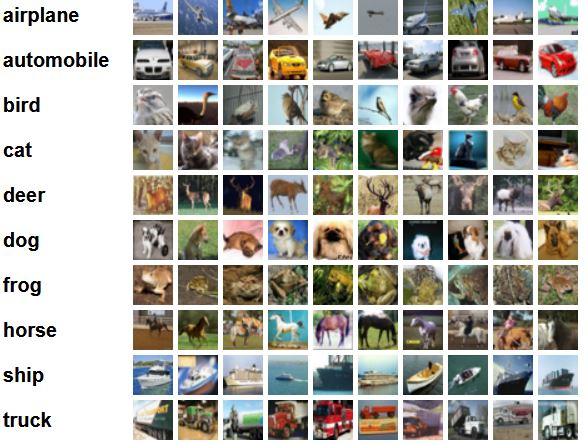
\includegraphics[scale=0.8]{CIFAR10}
    \caption{Ten examples of each class in the CIFAR10 dataset. }
\end{figure}
This dataset has $50.000$ samples for training and $10.000$ for test. The test batch contains the same number of examples of each of the $10.000$ classes in the dataset, that is, it contains $1.000$ examples of each class. 

It is important to remark that the classes are \emph{completely mutually exclusive}. That means that there is no overlap between the classes even if they have similar images, such as \emph{Cars} and \emph{Truck}, which are two of the classes of the dataset.

\section{Tensorflow}



Tensorflow\footnotemark is an open source library for developing machine learning frameworks.  

\begin{wrapfigure}{r}{5cm}
    \caption{Tensorflow logo.}
    
\includegraphics[scale=0.2]{tf-logo}
\end{wrapfigure}

%------------- Footnotemark
\footnotetext{Tensorflow documentation can be found at \url{https://www.tensorflow.org/}.}
%----------------------



It can be used for many tasks, but it focuses on training and inference of deep neural networks. It is used for both research and production at \emph{Google}, since it was also developed by the \emph{Google Brain} team for internal use. However, it was later released as open source.

The creation of new models is very simple, offering multiple abstraction levels. This is why it is suitable for our experiments. Also, the code is most of the times easily understandable.

There are other libraries that are widely used in machine learning algorithm development, such as \emph{PyTorch} or \emph{Jax}. However, Tensorflow has been chosen because I was a little bit more familiarized than with the other and because of its simplicity and how common it is. 

There are a few ways to define a NN or a framework using tensorflow. The most classic one is defining a sequential model using \lstinline{Keras}, a tensorflow API that defines layers of a neural network and helps with the implementation of simple NN structures. Let us see how to implement a very simple example of a NN with three \emph{Dense} layers: 

\begin{minted}[mathescape,linenos]{python}
model = keras.Sequential(
    [
        layers.Dense(2, activation="relu", name="layer1"),
        layers.Dense(3, activation="relu", name="layer2"),
        layers.Dense(4, name="layer3"),
    ]
)
\end{minted}

Another way of creating models using tensorflow is by defining a single step of training using \lstinline{tf.GradientTape()} and then executing the single step multiple times in a loop. Using GradientTape , tensorflow performs automatic differentiation, which is needed for the minimization process. Let us see the simplest example, consider the function $f(x) = x^2$, and imagine that we want to obtain $f'(3)$. We can obtain it using \lstinline{tf.GradientTape()} as follows:

\begin{minted}[mathescape,linenos]{python}
x = tf.constant(3.0)
with tf.GradientTape() as g:
  g.watch(x)
  y = x * x
dy_dx = g.gradient(y, x)
\end{minted}

In our case, the gradient is obtained and the applied to the optimizer by using:

\begin{minted}[mathescape,linenos]{python}
with tf.GradientTape() as tape:
    grads = tape.gradient(loss, model.trainable_variables)
    optimizer.apply_gradients(zip(grads, model.trainable_variables))
\end{minted}


\subsection{Tensorboard}

Tensorboard is a Tensorflow's visualization kit. It provides the visualization and tooling needed for machine learning experimentation. Among its more important utilities, we can find:
\begin{itemize}
\item Tracking and visualizing metrics (such as loss, accuracy, entropy) not only during the training but also when the training time has ended.

\item Visualizing the model graph: ops and layers.

\item Visualizing histograms of weights, biases and how tensors change during the training.

\item Projecting high-dimensional data to a lower dimensional space.

\item Displaying images,text and audio data.
\end{itemize}

Also, it is very easy to integrate with tensorflow.  Actually, in most of the cases it is as simple as adding the following \emph{callback} when we fit the model:

\begin{minted}[mathescape,linenos]{python}
    tensorboard_callback = tf.keras.callbacks.TensorBoard
                        (log_dir=log_dir, histogram_freq=1)
    model.fit(x=x_train, y=y_train, 
              epochs=5, 
              validation_data=(x_test, y_test),
              # The added callback produces the magic! 
              callbacks=[tensorboard_callback])  
\end{minted}

In our case, there are some differences, since we are not using the standard \lstinline{fit} function to train our models. Because of this, we have to log the information that we have obtained in each step. To do this, we can use the \lstinline{metrics} python package to group them (as it is done in the SimCLR code), or we can just directly save the information creating a \emph{file writer} and writing the desired variables on this file. We do this in the modification that we have done to BYOL's original code as follows:

\begin{minted}[mathescape,linenos]{python}
train_summary_writer = tf.summary.create_file_writer(args.log_dir)
with train_summary_writer.as_default():
    tf.summary.scalar('top_1_acc',float(acc),step=epoch)
    tf.summary.scalar('top_5_acc',float(top_5_acc),step=epoch)
    tf.summary.scalar('loss', float(losses[-1]), step=epoch)
\end{minted}


\section{Metrics}

As we have seen, firstly, our models create a representation of the input image and then this representation is evaluated using a supervised linear head. This is the most interesting part, since we can see if the representation obtained was really useful for the classification task. We need to present the measures that we will use to measure how good the representations that we are producing are.



\begin{notation}
We will address the \emph{true positives} (the positive samples of a class classified correctly) as $TP$, the \emph{true negatives} (the negative samples classified correctly) as $TN$, the \emph{false positives} (the negative samples classified as positive ones, which is a mistake of our model) as $FP$ and the false negatives (the positive samples classified incorrectly as negative samples) as $FN$.
\end{notation}

Using this notation, the measures that we will be using are the following:

\begin{itemize}
\item \emph{Accuracy}. The classic measure for models. It measures the number of successes our network has obtained producing the correct label for the representation created during the unsupervised part of the network. Formally,
\[
\operatorname{Accuracy} = \frac{TP + TN}{TP + TN + FP + FN}  .  
\] 
In SimCLR, we wil use two kinds of accuracies:
\begin{enumerate}
\item \emph{Top1} accuracy, which is the ordinary accuracy.
\item \emph{Top5} accuracy, which measures if any of the 5 highest probability answers matches the true label.
\end{enumerate}
\end{itemize}




